\section{Multi-output Gaussian Process model via Neural network}

\begin{figure}[!htb]
    \centering
    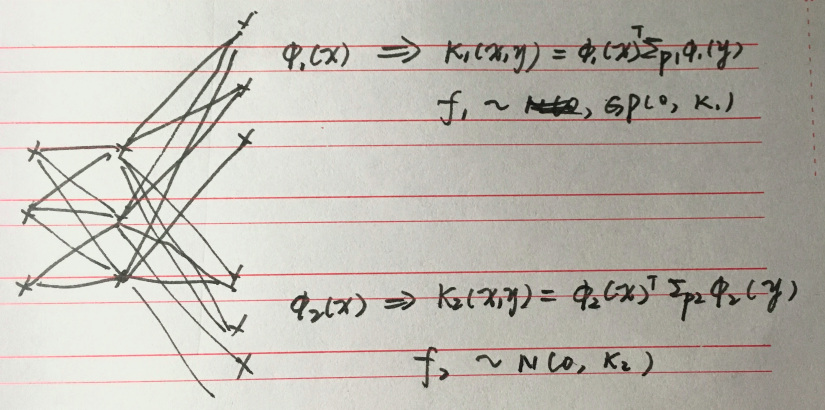
\includegraphics[width=\columnwidth]{./img/NN-MOGP.png}
    \caption{Architecture of the multi-output Gaussian process model.}
    \label{fig:MONNGP}
\end{figure}

We have shown that a GP can be constructed from a neural network with finite hidden units in the last layer. Now, we will show how to model the correlations between tasks and how to construct a multi-output Gaussian process model based on neural network.

Suppose we have $N$ observations $D_Q = \{X, Y | X \in R^{D \times N}, Y \in R^{N \times Q}\}$, we assume they are generated by $Q$ latent functions and polluted by noises with different noise level. Instead of building $Q$ independent models, we build a multi-output model that makes use of the correlations between the $Q$ tasks. Firstly, a neural network is used to define a \emph{shared feature map} $\phi_s : R^D \rightarrow R^{M_s}$. Then, for each task $i \in \{1,~\dots~,Q\}$, the shared feature $\phi_s(\bm{x})$ is followed by a \emph{task-specific} neural network that defines a feature map $\phi_i : R^{M_s} \rightarrow R^{M_i}$. We assume the $i$-th latent function $f_i(\bm{x})$ follows a GP distribution $f_i \sim \mathcal{GP}(0, k_i)$ defined as follows:

\begin{equation}
    \label{eq:mo_kernel}
    \left\{
    \begin{array}{lll}
        y_i                 &=&    f_i(\bm{x}) + \epsilon_i  \\
        f_i                 &\sim& \mathcal{GP}(0, k_i)      \\
        \epsilon_i          &\sim& N(0, \sigma_{n, i}^2)     \\
        k_i(\bm{x}, \bm{y}) &=&    \phi_i(\phi_s(\bm{x}))^T~\frac{\sigma_{p, i}^2}{M_i}~\phi_i(\phi_s(\bm{y}))
    \end{array}
    \right.
\end{equation}

As illustrated in \Fref{fig:MONNGP}, by defining GP with kernel function of \Fref{eq:mo_kernel}, we actually defined a neural network architecture with shared layers and task-specific layers, which is a common architecture used in multi-task deep learning \cite{ruder2017overview}. The correlations between tasks are naturally encoded by the shared layers, while the task-specific features are further learnt from the shared features.

With the model define in \Fref{eq:mo_kernel}, different tasks are \emph{conditionally independent} given the shared features, each specific task still sees a neural network with the same architecture plotted in \Fref{fig:NNGP}. The inferences of $\mu(\bm{x})$ and $\sigma^2(\bm{x})$ are exactly the same as \Fref{eq:DegeneratePred}, and no additional overhead will be introduced. As different tasks are conditionally independent, the log likelihood of the training data can be expressed as the sum of the log likelihood of each specific task
\begin{equation}
    \label{eq:mo_likelihood}
    \log p(Y | X, \bm{\Theta}) = \sum_{i=1}^Q \log p(\bm{y}_i | X, \bm{\theta}_i, \bm{\theta}_s),
\end{equation}
where $\bm{y}_i$ is the $i$-the column of $Y$, $\bm{\Theta}$ is the vector of all the parameters, including the shared parameters and the task-specific parameters. $\bm{\theta_i}$ is the vector of parameters for specific task $i$, including the weights of the $i$-th task-specific neural network, the weight prior factor $\sigma_{p, i}$ and the noise level $\sigma_{n, i}$ for the $i$-th task. $\bm{\theta}_s$ is a vector of the weights of the shared layers. The parameters $\bm{\Theta}$ are obtained by maximizing the likelihood function in \Fref{eq:mo_likelihood} with gradient back-propagation. The model averaging technique as described in subsection \ref{sec:deepensemble} is also employed in our model to improve the quality of uncertainty estimation. $K$ independent neural network models are trained with random initializations in our model. According to \Fref{eq:GPloglikelihood}, the time complexity of prediction for our model is $O(KN\sum_i^Q M_i^2)$.
